\pagecolor{CadetBlue!70!green}
\chapter{Steuerung komplexer Informatik-Systeme}

Mit den vielen Bauteilen, die nun zur Verfügung stehen, lassen sich bereits große und komplexe Projekte realisieren. Um dabei nicht den Überblick zu verlieren, hilft es, sich mit einigen weiteren Konzepten aus der Informatik zu beschäftigen, die das Programm und die Vorgehensweise zur Erstellung des Programms besser strukturieren.

In diesem Kapitel lernst du...
\begin{itemize}
	\item \dots die Funktionsweise von Programmen mit einem Zustandsdiagramm zu planen und zu veranschaulichen,
	\item \dots Programme durch eine zustandsbasierte Modellierung als endlicher Automat zu flexibilisieren.
\end{itemize}

\bigskip

\begin{projektueberblick}
	\item Fußgängerampel \dotfill \pageref{proj:fussgaengerampel}
	\item Parkplatzschranke \dotfill \pageref{proj:parkplatzschranke}
\end{projektueberblick}

\newpage
\nopagecolor

\section{Automaten}
% Aufzug als Beispiel (siehe Wikipedia) // Stoppuhr am Smartphone mit Arduino und LCD nachbauen (Startbildschirm, zählend, stopbildschirm als Zustände, Übergänge durch Knopf gesteuert; erste Aufgabe: a) angefangenes Programm erweitern, b) zustände für Timer aufschreiben c) Timer programmieren
% ODER: einfacher Kaugummiautomat (Zustände: Kaugummiauswahl, Geldeingabe, Kaugummiausgabe)

% Zustände bei Menüführung auf LCD mit drei Tastern (runter/hoch/bestätigen)

% Zustände bei Ampelschaltung, Erweiterung: mit Fußgängerampel

% Aufbau
% bis jetzt Algorithmen als feste Handlungsabfolgen beschrieben, nun zustandsbasierte Programmierung
% Zustandsdiagramm vorgeben und erläutern lassen
% Begriffe: Zustand, auslösende Aktion, Bedingung, ausgelöste Aktion

% am Ende abstrahieren: Endlicher Automat mit endlich vielen Zuständen, Eingaben (auslösende Aktion + Bedingung), Überführungsfunktion, Startzustand und endlich vielen Endzuständen

Bisher wurden Algorithmen rezeptartig als feste Handlungsabfolgen beschrieben, die nacheinander durchlaufen werden und dabei ggf. einfache Fallunterscheidungen berücksichtigen. In der Automatentheorie steht weniger das Befolgen eines Rezeptes im Mittelpunkt als das Einnehmen verschiedener Zustände, zwischen denen unter festgelegten Bedingungen Übergänge stattfinden. Dies macht die Algorithmen flexibler im Umgang mit Eingaben aus der Umwelt, wodurch sie zudem leichter zu erweitern sind.

\begin{ziel}
	\textbf{Ziel:} Durch eine zustandsbasierte Modellierung sollen Algorithmen flexibler werden und einfacher zu erweitern. 
\end{ziel}

\begin{aufgabe} \emph{Ampelzustände}
	\begin{enumerate}[label=\alph*), itemsep=0mm, parsep=0mm]
		\item Nenne die vier Zustände (\emph{engl. states}) einer Ampel. Beschreibe die Bedingung(en), unter denen der Wechsel vom einen in den nächsten Zustand stattfindet.
		\item Unten ist ein sogenanntes Zustandsdiagramm einer Ampel zu sehen. Erläutere, wie es aufgebaut ist und ordne ihnen die vier Ampelzustände zu.
		
		\emph{Hinweis: s: state (engl. für Zustand), t: time (engl. für Zeit)}
		\begin{figure}[H]
			\centering
			\begin{tikzpicture}[every state/.style={fill=CadetBlue!70!green, draw=black, thick, text={black}, font=\sffamily},node distance = 5cm, shorten >= 1pt, on grid, auto, initial text={},>=stealth']
			\node[state, initial] (z0)  {\parbox{2cm}{\centering \rule{1.5cm}{0mm} \rule{2cm}{0.25mm}  $s=0$}};
			\node[state] (z1) [right = of z0] {\parbox{2cm}{\centering \rule{1.5cm}{0mm} \rule{2cm}{0.25mm}  $s=1$}};
			\node[state] (z2) [below = of z1] {\parbox{2cm}{\centering \rule{1.5cm}{0mm} \rule{2cm}{0.25mm}  $s=2$}};
			\node[state] (z3) [left = of z2] {\parbox{2cm}{\centering \rule{1.5cm}{0mm} \rule{2cm}{0.25mm}  $s=3$}};
			\path[->, thick] (z0) 	edge 				node {$t \geq 60s$} (z1)
									edge [loop above] 	node {$t < 60s$} ()
							(z1) 	edge				node {$t \geq 2s$} (z2)
									edge [loop above] 	node {$t<2s$} ()
							(z2) 	edge				node {$t \geq 60s$} (z3)
									edge [loop below] 	node {$t<60s$} ()
							(z3) 	edge				node {$t \geq 8s$} (z0) 
									edge [loop below] 	node {$t<8s$} ();
			\end{tikzpicture}
		\end{figure} 
		\item Unten ist abgebildet, wie ein Programm aussehen könnte, das das Zustandsdiagramm modelliert. Jeder Übergang (jede Bedingung) wird durch eine \texttt{falls}-Abfrage in das Programm integriert. Vervollständige das Programm zur Modellierung einer einfachen Ampel und baue die Ampel auf.
		
		\emph{Erweiterung:} Programmiere jeden Ampelzustand als eigene Funktion, sodass das Programm lesbarer wird.
		\begin{figure}[H]
			\centering
			\includegraphics[width=0.85\textwidth]{./pics/ampel-automat-start.png}
		\end{figure} 
	\end{enumerate}
	{\scriptsize\emph{Idee: Materialien zum Kerncurriculum Informatik im Sekundarbereich I, Niedersächsisches Kultusministerium}}
\end{aufgabe}

Bei einer klassischen Programmierung mit \texttt{warte}-Blöcken wäre eine Erweiterung um eine Fußgängerampel, die zu jedem beliebigen Zeitpunkt aktiviert werden kann, unmöglich, da das Programm während des Wartens das Drücken der Fußgängerampel gar nicht mitbekommen würde. Durch die zustandsbasierte Modellierung mithilfe einer Stoppuhr lässt sich die Fußgängerampel jedoch integrieren. 

\begin{projekt}{Erweiterung um eine Fußgängerampel}\label{proj:fussgaengerampel}
	
	\bigskip
	\begin{minipage}{0.6\textwidth}
		Eine Fußgängerampel ist zunächst aus oder deaktiviert. Sie kann jederzeit durch einen Taster aktiviert werden, das heißt, sie zeigt rot. Sie bleibt solange rot, bis die normale Ampel ebenfalls rot zeigt und eine gewisse Mindestdauer vergangen ist. Die normale Ampel bleibt nun rot, während die Fußgängerampel auf grün springt. Nach einer gewissen Zeit schaltet die Fußgängerampel wieder auf rot. Nach ein paar Sekunden Rotphase für die letzten Fußgänger, die ihren Weg über die Straße noch beenden müssen, ist die Fußgängerampel wieder aus und die normale Ampel springt in die Rot-Gelb-Phase, mit der sie ihren normalen Rhythmus fortsetzt.
	\end{minipage}
	\hfill
	\begin{minipage}{0.38\textwidth}
		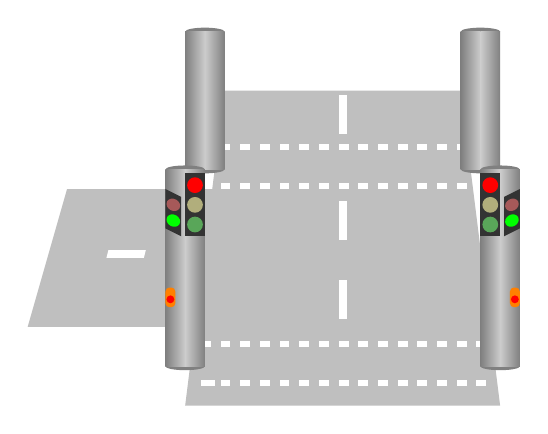
\begin{tikzpicture}[scale=0.5]
		%Seitenstraße
		\fill[gray!50] (-4,1) -- (2,1) -- (2,4.5) -- (-3,4.5) -- cycle;
		\fill[white] (-2,2.75) -- ++(0.95,0) -- ++(0.05,0.2) -- ++(-0.95,0) -- cycle;
		%Hauptstraße
		\fill[gray!50] (0,-1) -- (8,-1) -- (7,7) -- (1,7) -- cycle;
		\fill[white] (3.9,1.2) rectangle ++(0.2,1);
		\fill[white] (3.9,3.2) rectangle ++(0.2,1);
		\fill[white] (3.9,5.9) rectangle ++(0.2,1);
		\foreach \x in {0.4,0.9,...,7.4} {
			\fill[white] (\x,-0.5) rectangle ++(0.25,0.15);
			\fill[white] (\x,0.5) rectangle ++(0.25,0.15);
			\fill[white] (\x,4.5) rectangle ++(0.25,0.15);
			\fill[white] (\x,5.5) rectangle ++(0.25,0.15);
		}
		\fill[white] (0.5,-0.5) rectangle ++(0.25,0.15);
		% Säule links hinten
		\fill[gray] (0.5,5) ellipse [x radius=0.5, y radius=0.1];
		\fill[gray] (0.5,8.5) ellipse [x radius=0.5, y radius=0.1];
		\shade [left color=gray, right color=gray!40] (0,5) rectangle ++(0.5,3.5);
		\shade [left color=gray!40, right color=gray] (0.5,5) rectangle ++(0.5,3.5);
		% Säule rechts hinten
		\fill[gray] (7.5,5) ellipse [x radius=0.5, y radius=0.1];
		\fill[gray] (7.5,8.5) ellipse [x radius=0.5, y radius=0.1];
		\shade [left color=gray, right color=gray!40] (7,5) rectangle ++(0.5,3.5);
		\shade [left color=gray!40, right color=gray] (7.5,5) rectangle ++(0.5,3.5);
		% Säule links
		\fill[gray] (0,0) ellipse [x radius=0.5, y radius=0.1];
		\fill[gray] (0,5) ellipse [x radius=0.5, y radius=0.1];
		\shade [left color=gray, right color=gray!40] (-0.5,0) rectangle ++(0.5,5);
		\shade [left color=gray!40, right color=gray] (0,0) rectangle ++(0.5,5);
		% große Ampel links
		\fill[black!80] (0,3.3) rectangle ++(0.5,1.6);
		\fill[red] (0.25,4.6) circle [radius=2mm];
		\fill[yellow!30!gray] (0.25,4.1) circle [radius=2mm];
		\fill[green!30!gray] (0.25,3.6) circle [radius=2mm];
		%Fußgängerampel links
		\fill[black!80] (-0.5,3.5) -- ++(0.4,-0.2) -- ++(0,1) -- ++ (-0.4,0.2) -- cycle;
		\fill[red!30!gray] (-0.3,4.1) ellipse [x radius=1.8mm, y radius=1.5mm,rotate=-30];
		\fill[green] (-0.3,3.7) ellipse [x radius=1.8mm, y radius=1.5mm,rotate=-30];
		\fill[orange,rounded corners=0.5mm] (-0.5,1.5) rectangle ++(0.25,0.5);
		\fill[red] (-0.375,1.7) circle [radius=1mm];
		% Säule rechts
		\fill[gray] (8,0) ellipse [x radius=0.5, y radius=0.1];
		\fill[gray] (8,5) ellipse [x radius=0.5, y radius=0.1];
		\shade [left color=gray, right color=gray!40] (7.5,0) rectangle ++(0.5,5);
		\shade [left color=gray!40, right color=gray] (8,0) rectangle ++(0.5,5);
		\fill[orange,rounded corners=0.5mm] (8.25,1.5) rectangle ++(0.25,0.5);
		\fill[red] (8.375,1.7) circle [radius=1mm];
		% große Ampel rechts
		\fill[black!80] (7.5,3.3) rectangle ++(0.5,1.6);
		\fill[red] (7.75,4.6) circle [radius=2mm];
		\fill[yellow!30!gray] (7.75,4.1) circle [radius=2mm];
		\fill[green!30!gray] (7.75,3.6) circle [radius=2mm];
		%Fußgängerampel rechts
		\fill[black!80] (8.1,3.3) -- ++(0.4,0.2) -- ++(0,1) -- ++ (-0.4,-0.2) -- cycle;
		\fill[red!30!gray] (8.3,4.1) ellipse [x radius=1.8mm, y radius=1.5mm,rotate=30];
		\fill[green] (8.3,3.7) ellipse [x radius=1.8mm, y radius=1.5mm,rotate=30];
		\end{tikzpicture}
	\end{minipage}

	\begin{enumerate}[label=\alph*), itemsep=0mm, parsep=0mm]
		\item Entnimm der obigen Beschreibung die vier Zustände einer Fußgängerampel und die Bedingungen, unter denen vom einen Zustand in den nächsten gewechselt wird. Entwickle daraus ein Zustandsdiagramm für die Fußgängerampel. Ergänze die Übergänge von der Rotphase der normalen Ampel zur Rotphase der Fußgängerampel und von der (wieder) deaktivierten Fußgängerampel zur Rot-Gelb-Phase der normalen Ampel.
		
		\emph{Achtung:} Hier liegen zwei Automaten vor, nämlich die normale Ampel und die Fußgängerampel, daher gibt es auch zwei Startzustände.
		
		\item Ergänze die Fußgängerampel inkl. Taster auf dem Steckbrett und ergänze das Programm um die Zustände der Fußgängerampel.
		
		\emph{Tipp:} Nutze eine Variable, um den Tasterstatus zu speichern, nachdem der Taster einmal gedrückt wurde.
	\end{enumerate}
	{\scriptsize\emph{Idee: Materialien zum Kerncurriculum Informatik im Sekundarbereich I, Niedersächsisches Kultusministerium}}
\end{projekt}
\marginpar{%
	\footnotesize%
	\zurueck
	\hyperref[abb:tasterkonfiguration]{Taster \\auslesen}
}

\begin{zsfg}{Endlicher Automat und Zustandsdiagramm}
	Ein Automat (auch: abstrakte Maschine) ist in der Informatik ein Modell zur Beschreibung einer Datenverarbeitung. 
	Er befindet sich anfangs in seinem Startzustand. Abhängig von der nächsten Eingabe (z.\,B. das Ablaufen einer Zeit oder das Drücken eines Tasters) und des aktuellen Zustands erfolgt der Übergang in einen Folgezustand. Auch zu diesem gibt es wiederum einen Folgezustand, der abhängig von der nächsten Eingabe und dem aktuellen Zustand erreicht wird. Es kann einen oder mehrere Endzustände geben, die keinen Folgezustand haben, wenn der Ablauf des Automaten vollständig ausgeführt wurde. Wenn der Automat endlich viele Zustände hat, spricht man von einem \textbf{endlichen Automaten}.
	
	Ein Zustandsdiagramm veranschaulicht das Verhalten eines Automaten. Die Zustände werden mit einem Kreis oder abgerundeten Rechteck dargestellt. Die Übergänge werden mit Pfeilen dargestellt, an denen die Bedingung für den Übergang steht. Der Startzustand wird mit einem zusätzlichen Pfeil markiert, an den manchmal zusätzlich \texttt{start} geschrieben wird. Der ggf. vorhandene Endzustand wird durch einen doppelten Rahmen markiert.
	
	\begin{figure}[H]
		\centering
		\begin{tikzpicture}[every state/.style={fill=CadetBlue!70!green, draw=black, thick, text={black}, font=\sffamily},node distance = 2cm, shorten >= 1pt, on grid, auto, initial text={start},>=stealth']
		\node[state, initial] (z0)  {$s=0$};
		\node[state] (z1) [above right = of z0] {$s=1$};
		\node[state] (z2) [below right = of z0] {$s=2$};
		\node[state,accepting] (z3) [below right = of z1] {$s=3$};
		\path[->, thick] (z0) 	edge 				node [above left] 	{bedingung1} (z1)
								edge 				node [below left] 	{bedingung2} (z2)
						(z1) 	edge				node [above right]	{bedingung3} (z3)
								edge [loop above] 	node 				{bedingung4} ()
						(z2) 	edge				node [below right]	{bedingung5} (z3)
								edge [loop below] 	node 				{bedingung6} ();
		\end{tikzpicture}
	\end{figure}
\end{zsfg}

\newpage
\begin{projekt}{Parkplatzschranke} \label{proj:parkplatzschranke}
	
	Auf einen Parkplatz kommt man häufig erst, wenn man einen Parkschein gezogen hat. Danach öffnet sich die Schranke und man kann auf den Parkplatz fahren. Die Schranke schließt sich automatisch wieder, nachdem das Auto hindurchgefahren ist. Beim Verlassen des Parkplatzes muss man wiederum zuerst den bezahlten Parkschein einlesen lassen, bevor sich die Schranke öffnet und automatisch wieder schließt, nachdem ein Auto hindurchgefahren ist.
	
	\begin{figure}[H]
		\centering
		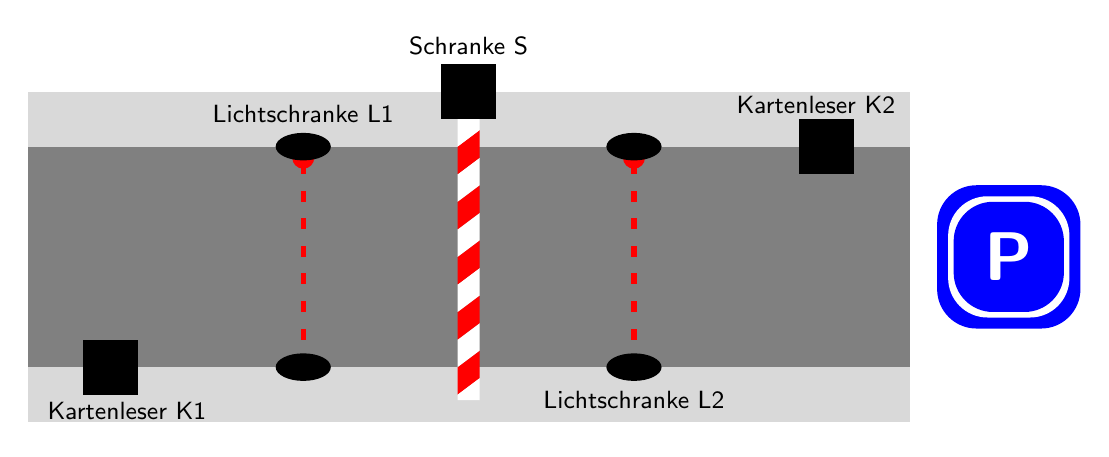
\begin{tikzpicture}[scale=0.7]
		%Straße
		\fill[gray!30] (0,0) rectangle (16,1);
		\fill[gray] (0,1) rectangle (16,5);
		\fill[gray!30] (0,5) rectangle (16,6);
		%Kartenleser
		\fill[black] (1,0.5) rectangle ++(1,1) node at (1.8,0.2)  {\sffamily\small Kartenleser K1};
		\fill[black] (14,4.5) rectangle ++(1,1) node at (14.3,5.75) {\sffamily\small Kartenleser K2};
		%Lichtschranke 1
		\fill[black] (5,1) ellipse [x radius=0.5, y radius=0.25];
		\fill[red] (5,4.8) circle [radius=0.2];
		\fill[black] (5,5) ellipse [x radius=0.5, y radius=0.25] node at (5,5.6) {\sffamily\small Lichtschranke L1};
		\foreach \y in {1.5, 2, ..., 4.5} {
			\fill[red] (4.95,\y) rectangle ++(0.1,0.2);
		}
		%Lichtschranke 2
		\fill[black] (11,1) ellipse [x radius=0.5, y radius=0.25];
		\fill[red] (11,4.8) circle [radius=0.2];
		\fill[black] (11,5) ellipse [x radius=0.5, y radius=0.25] node at (11,0.4) {\sffamily\small Lichtschranke L2};
		\foreach \y in {1.5, 2, ..., 4.5} {
			\fill[red] (10.95,\y) rectangle ++(0.1,0.2);
		}
		%Schranke
		\foreach \y in {0.5,1.5,...,4.5} {
			\fill[red] (7.8,\y) -- ++(0.4,0.3) -- ++(0,0.5) -- ++(-0.4,-0.3) -- cycle;
			\fill[white] (7.8,\y+0.5) -- ++(0.4,0.3) -- ++(0,0.5) -- ++(-0.4,-0.3) -- cycle;
		}
		\fill[white] (7.8,0.4) -- ++(0.4,0) -- ++(0,0.4) -- ++(-0.4,-0.3) -- cycle;
		\fill[black] (7.5,5.5) rectangle ++(1,1) node at (8,6.5) [above] {\sffamily\small Schranke S};
		% Parkplatzzeichen
		\fill [blue, rounded corners=0.5cm] (16.5,1.7) rectangle ++(2.6,2.6);
		\fill [white, rounded corners=0.5cm] (16.7,1.9) rectangle ++(2.2,2.2);
		\fill [blue, rounded corners=0.5cm] (16.8,2) rectangle ++(2,2) node at ++(-1,-1) {\Huge\color{white}\sffamily \bfseries P};
		\end{tikzpicture}
	\end{figure}
	
	\medskip
	Das Verhalten der Parkplatzschranke soll auf dem Steckbrett simuliert werden. Dazu wird aus Pappe ein \enquote{Auto} geschnitten, das durch die mittlere Spalte des Steckbretts \enquote{fährt}.
	
	\begin{enumerate}[label=\alph*), itemsep=0mm, parsep=0mm]
		\item Erläutere, wie man die Kartenleser und das Durchfahren der Schranke mithilfe von zwei Tastern und zwei Lichtschranken simulieren kann. Notiere alle benötigten Bauteile.
		\item Baue die Parkplatzschranke mit allen benötigten Teilen auf dem Steckbrett auf.
		\item Entwickle ein Automatenmodell für die Parkplatzschranke. Überlege dazu, in welchen Zuständen sich die einzelnen Elemente beim Einfahren und beim Ausfahren befinden.
		%TODO: Anfang vorgeben?
		\item Implementiere das Automatenmodell.
	\end{enumerate}
	{\scriptsize\emph{Idee: Materialien zum Kerncurriculum Informatik im Sekundarbereich I, Niedersächsisches Kultusministerium}}
\end{projekt}
\marginpar{%
	\footnotesize%
	\zurueck% 
	\hyperref[abb:tasterkonfiguration]{Taster}\\
	\zurueck% 
	\hyperref[abb:schaltplan-ldr]{LDR}\\
	\zurueck% 
	\hyperref[sec:servo]{Servo}
}

%TODO: Abschnitt Steuern und Regeln hinzufügen
%\newpage
%\section{Steuern und Regeln}
%%Einstiegsbeispiel: Der schon gebaute Badezimmerlüfter - durch das Anspringen des Lüfters wird die Luftfeuchtigkeit wieder heruntergeregelt
%
%% Solarzellen-Nachsteuerung (mit LDR und Servo Richtung Lampe ausrichten)

\vfill
\begin{links}
	\item \href{https://www.instructables.com/id/6-Shooter-Arduino-Drink-Mixing-Station/}{Cocktail Mixer}
	
	Dieser Automat mixt automatisch einen aus sechs wählbaren Drinks!
	
	\item \href{https://blog.arduino.cc/2014/07/17/a-low-cost-robotic-hand-tutorial-mirroring-your-own-fingers/}{Roboterhand}
	
	Mit diesem Aufbau wird die eigene Hand auf eine Roboterhand gespiegelt, wodurch sich der Roboter viel besser steuern lässt.
	
	\item \href{http://oneaerospace.com/index.html}{One | Aerospace}
	
	Diese Gruppe von Studenten versucht u. a. mit Hilfe eines Arduino eine Rakete zu bauen!
	
	\item \href{https://www.heise.de/make/meldung/Elektronikbasteleien-von-der-Farm-Ziegen-mit-GPS-auf-der-Spur-4340346.html}{Ziegen-Tracker}
	
	Mit dieser Kombination aus Arduino und GPS-Antenne wird es Ziegen unmöglich von ihrer Farm auszubrechen.
\end{links}